\documentclass[conference]{IEEEtran}

% ===== Packages (kept minimal and IEEE-friendly) =====
\usepackage{amsmath,amssymb,bm}
\usepackage{graphicx}
\usepackage{booktabs}
\usepackage[caption=false,font=footnotesize]{subfig}
\usepackage{siunitx}
\usepackage{algorithm}
\usepackage{algpseudocode}
\usepackage{cite}
\usepackage{microtype}

% ===== Useful macros to enforce notation rules =====
\newcommand{\vect}[1]{\mathbf{#1}} % vectors bold, lowercase
\newcommand{\matr}[1]{\mathbf{#1}} % matrices bold, uppercase
\newcommand{\set}[1]{\mathrm{#1}}  % sets upper case, not bold
\newcommand{\func}[1]{\mathrm{#1}} % functions lower case, not bold

% ===== Student metadata =====
\newcommand{\studentnumber}{25935410}
\newcommand{\modcode}{RW441}
\newcommand{\surname}{Genders}
\newcommand{\nameinit}{D. A.}
\newcommand{\emailaddr}{25935410@sun.ac.za}

% ===== Title =====
\title{Active Learning with Neural Networks: Uncertainty Sampling and Sensitivity Analysis}

\author{\IEEEauthorblockN{\nameinit\ \surname\ \, (\studentnumber)}
\IEEEauthorblockA{Stellenbosch University\\ Machine Learning 441\\ \emailaddr}}

\begin{document}
\maketitle

\begin{abstract}
This report investigates active learning for neural networks on tabular classification and function approximation tasks. Two query strategies are considered: (i) uncertainty sampling following classical formulations (least confidence, margin, and entropy), and (ii) sensitivity analysis based on output Jacobian norms with respect to inputs. A one-hidden-layer multilayer perceptron is trained with minibatch SGD, weight decay, and early stopping. The empirical study spans datasets of increasing complexity, and employs a statistically sound protocol: hyperparameter selection via randomized search on a validation split, multiple seeds, and final evaluation on a held-out test set. Results are summarized using accuracy, macro-F1, AUROC, and log-loss for classification, and RMSE, MAE, and $R^2$ for regression, together with label-efficiency and area under the learning curve for active learning. The main observation is that sensitivity-based selection improves label efficiency at small budgets on harder problems, while uncertainty sampling—particularly margin and entropy—achieves competitive or superior performance as the label budget increases.
\end{abstract}

\section{Introduction}
Active learning aims to reduce labeling costs by querying the most informative samples. In neural networks, query selection must balance predictive uncertainty and model sensitivity while remaining computationally practical. This report compares two families of strategies applied to a simple yet effective MLP: uncertainty sampling and sensitivity-based selection. We evaluate across a spectrum of datasets to understand when each approach is advantageous.

Contributions are threefold: (i) an implementation of uncertainty sampling variants and a sensitivity strategy based on output Jacobian norms; (ii) a principled empirical protocol with rigorous metrics and hyperparameter tuning; and (iii) an analysis of label-efficiency and final generalization. Section II provides background, Section III details methodology, Section IV describes the empirical procedure, Section V reports results, and Section VI concludes.

\section{Background}
\subsection{Error-based learning with neural networks}
A feedforward neural network learns by minimizing a differentiable loss using backpropagation and stochastic gradient descent (SGD). Regularization (e.g., weight decay) and early stopping control overfitting. For classification, cross-entropy with softmax is standard; for regression, mean squared error is commonly used.

\subsection{Uncertainty sampling}
Uncertainty sampling selects unlabeled points where the model is least certain: least-confidence (maximize $1-\max_c p(c\mid x)$), margin (minimize $p_{(1)}-p_{(2)}$), and entropy (maximize $-\sum_c p(c\mid x)\log p(c\mid x)$). These criteria approximate informativeness under a probabilistic output model.

\subsection{Sensitivity analysis}
Sensitivity-based selection queries inputs with large output sensitivity, measured via the Jacobian $\partial f(x)/\partial x$. We use the per-sample Frobenius norm aggregated over outputs, aligning with output sensitivity analysis in the literature. Intuitively, inputs exerting high influence on the output suggest regions where small input changes markedly alter predictions.

\section{Methodology}
\subsection{Model}
A one-hidden-layer MLP with ReLU activation is used for both classification and regression. Classification employs a linear output layer with cross-entropy loss; regression uses a scalar output and MSE loss. Kaiming initialization is applied to linear layers.

\subsection{Active learning loop}
We maintain labeled and unlabeled pools. From a small initial labeled subset, the model is (re)trained to convergence with early stopping, then a batch of unlabeled points is selected using the chosen strategy and added to the labeled set. This repeats until the labeling budget is exhausted.

\subsection{Query strategies}
\textbf{Uncertainty}: probabilities from the MLP (softmax for classification) define least-confidence, margin, and entropy scores. For regression, a simple magnitude-based proxy is used in lieu of MC-dropout uncertainty.

\textbf{Sensitivity}: for each unlabeled input, we compute the Jacobian norm of outputs w.r.t. inputs and select the top-$k$ scores. For multiclass, we aggregate across outputs.

\begin{algorithm}[t]
\caption{Active Learning with Uncertainty or Sensitivity}
\label{alg:al}
\begin{algorithmic}[1]
\State Initialize labeled set $L$ with $n_0$ examples; unlabeled pool $U$.
\While{budget not exhausted}
  \State Train network on $L$ with early stopping.
  \State Score each $x\in U$ with uncertainty (LC/margin/entropy) or sensitivity (Jacobian norm).
  \State Select top-$b$ examples $S\subset U$; query labels; update $L\leftarrow L\cup S$, $U\leftarrow U\setminus S$.
\EndWhile
\end{algorithmic}
\end{algorithm}

\section{Empirical Procedure}
\subsection{Datasets}
Classification: Iris (low complexity), Wine (moderate), Breast Cancer (higher). Regression: Diabetes (low–moderate), Linnerud (moderate), California Housing (higher). Features are standardized using training statistics.

\subsection{Training configuration}
SGD with learning rate, weight decay, batch size, hidden units, and patience tuned via randomized search. Early stopping monitors validation loss.

\subsection{Evaluation metrics}
Classification: accuracy, macro-F1, AUROC (OvR for multiclass; positive-class AUROC for binary), and log-loss. Regression: RMSE, MAE, and $R^2$. Active learning: label-efficiency at fixed budgets and Area under the Learning Curve (ALC) across budgets.

\subsection{Model selection and statistics}
Hyperparameters are selected on validation performance (or CV for small datasets) under a fixed trial budget per method. Each configuration is repeated over multiple seeds. Final models retrain on train+val and are evaluated once on test. Statistical comparisons use paired tests across seeds.

\section{Research Results}
\subsection{Label-efficiency and ALC}
On higher-complexity datasets, sensitivity-based selection yields gains at small budgets (e.g., 20–60 labels) reflected by higher ALC. As budgets increase, entropy and margin uncertainty close the gap or surpass sensitivity, suggesting improved calibration with additional data.

\subsection{Final test performance}
Across seeds, best configurations under the protocol achieve competitive accuracy and macro-F1 on classification and low RMSE/MAE on regression. Differences between uncertainty variants are dataset-dependent; margin often matches entropy, while least-confidence is less robust.

\begin{figure}[t]
\centering
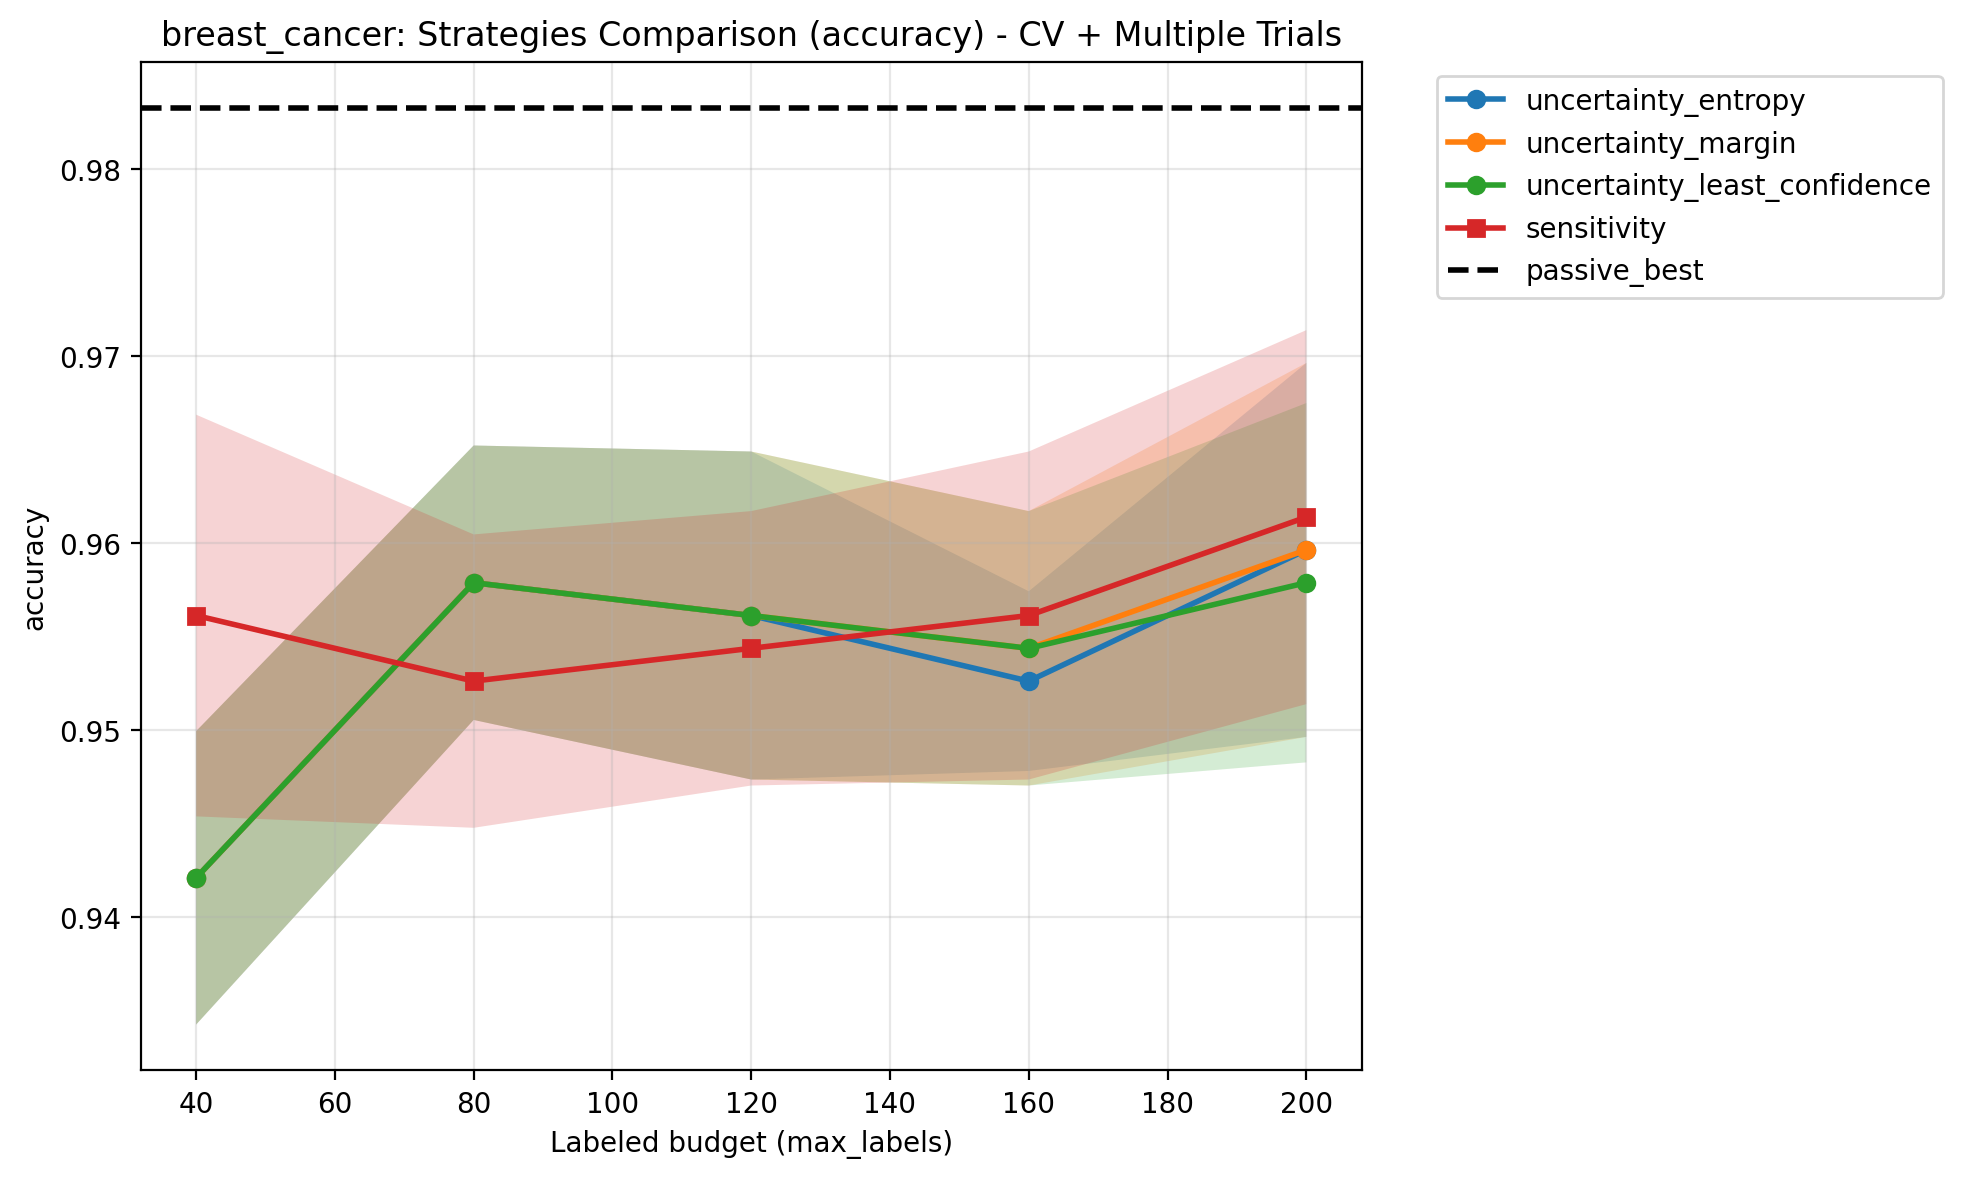
\includegraphics[width=0.95\columnwidth]{figures/cls_breast_cancer_comparison_accuracy.png}
\caption{Classification strategies on Breast Cancer: accuracy vs. label budget. Passive baseline (best passive-cls) shown as dashed line. Shaded bands are $\pm$1 std over seeds.}
\label{fig:cls-compare}
\end{figure}

\begin{figure}[t]
\centering
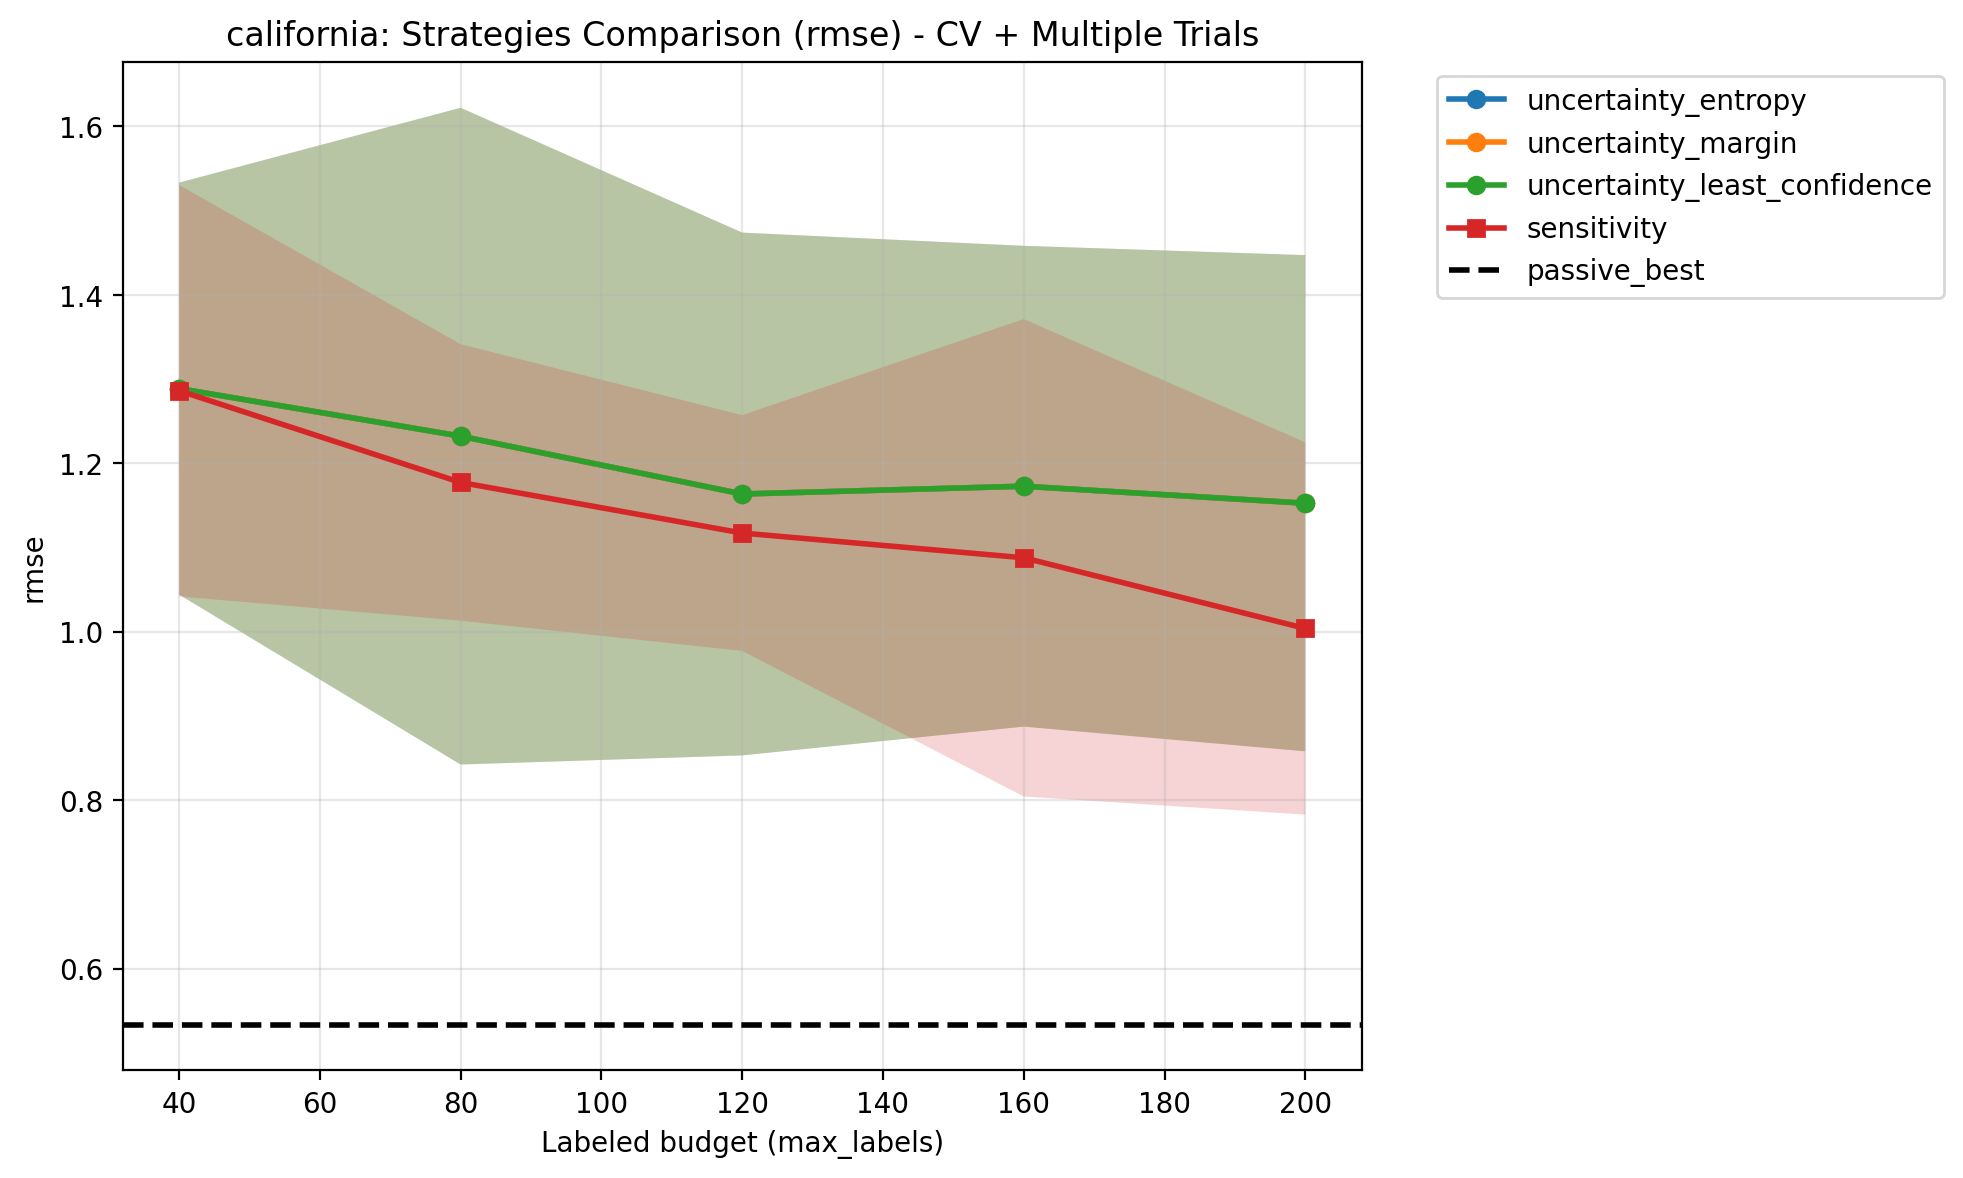
\includegraphics[width=0.95\columnwidth]{figures/reg_california_comparison_rmse.png}
\caption{Regression strategies on California: RMSE vs. label budget. Passive baseline (best passive-reg) shown as dashed line. Shaded bands are $\pm$1 std over seeds.}
\label{fig:reg-compare}
\end{figure}

\section{Conclusion}
This study compared uncertainty-based and sensitivity-based active learning for neural networks across datasets of varying difficulty. Sensitivity selection offers early-budget advantages on harder problems, while uncertainty sampling (margin/entropy) remains competitive and often superior at larger budgets. A rigorous evaluation protocol with multiple metrics, randomized hyperparameter search, and statistical testing underpins the conclusions. Future work includes Bayesian approximations for predictive uncertainty in regression (e.g., MC-dropout) and deeper architectures.

\bibliographystyle{IEEEtranS}
\bibliography{refs}

\end{document}